\section{自己紹介}
こんにちは、あわあわくん()(@materialofmouse)です。
同人誌を書く話になったのでLEDでひたすら発電してみました。
この章ではLEDで発電という普通はやらないことをやっています。
それに検証性がないのでちゃんと書かれてません。おまけだとおもって読んでください。

\subsection{LEDで発電できるの?}
できます。
詳しい話はインターネットで出てきますので、興味があるかたはぜひ調べてみてください。

\subsection{実際にやってみる}
場所:近くの駐車場
時間:14:10
光源:太陽光
照度:160000lux
天気:雲ひとつない晴れ

\subsubsection{LED1個}
まず、LEDを1個。アノード側にテスターのプラス、カソード側にテスターのマイナスを接続します。
この状態でLEDを太陽の方へ向けてみます。そこで発生した電流と電圧の値を取っていきます。
手元の環境では、普通の白色LEDから約10uA,約1.2V発生しました。

\begin{figure}[htbp]
    \centering
    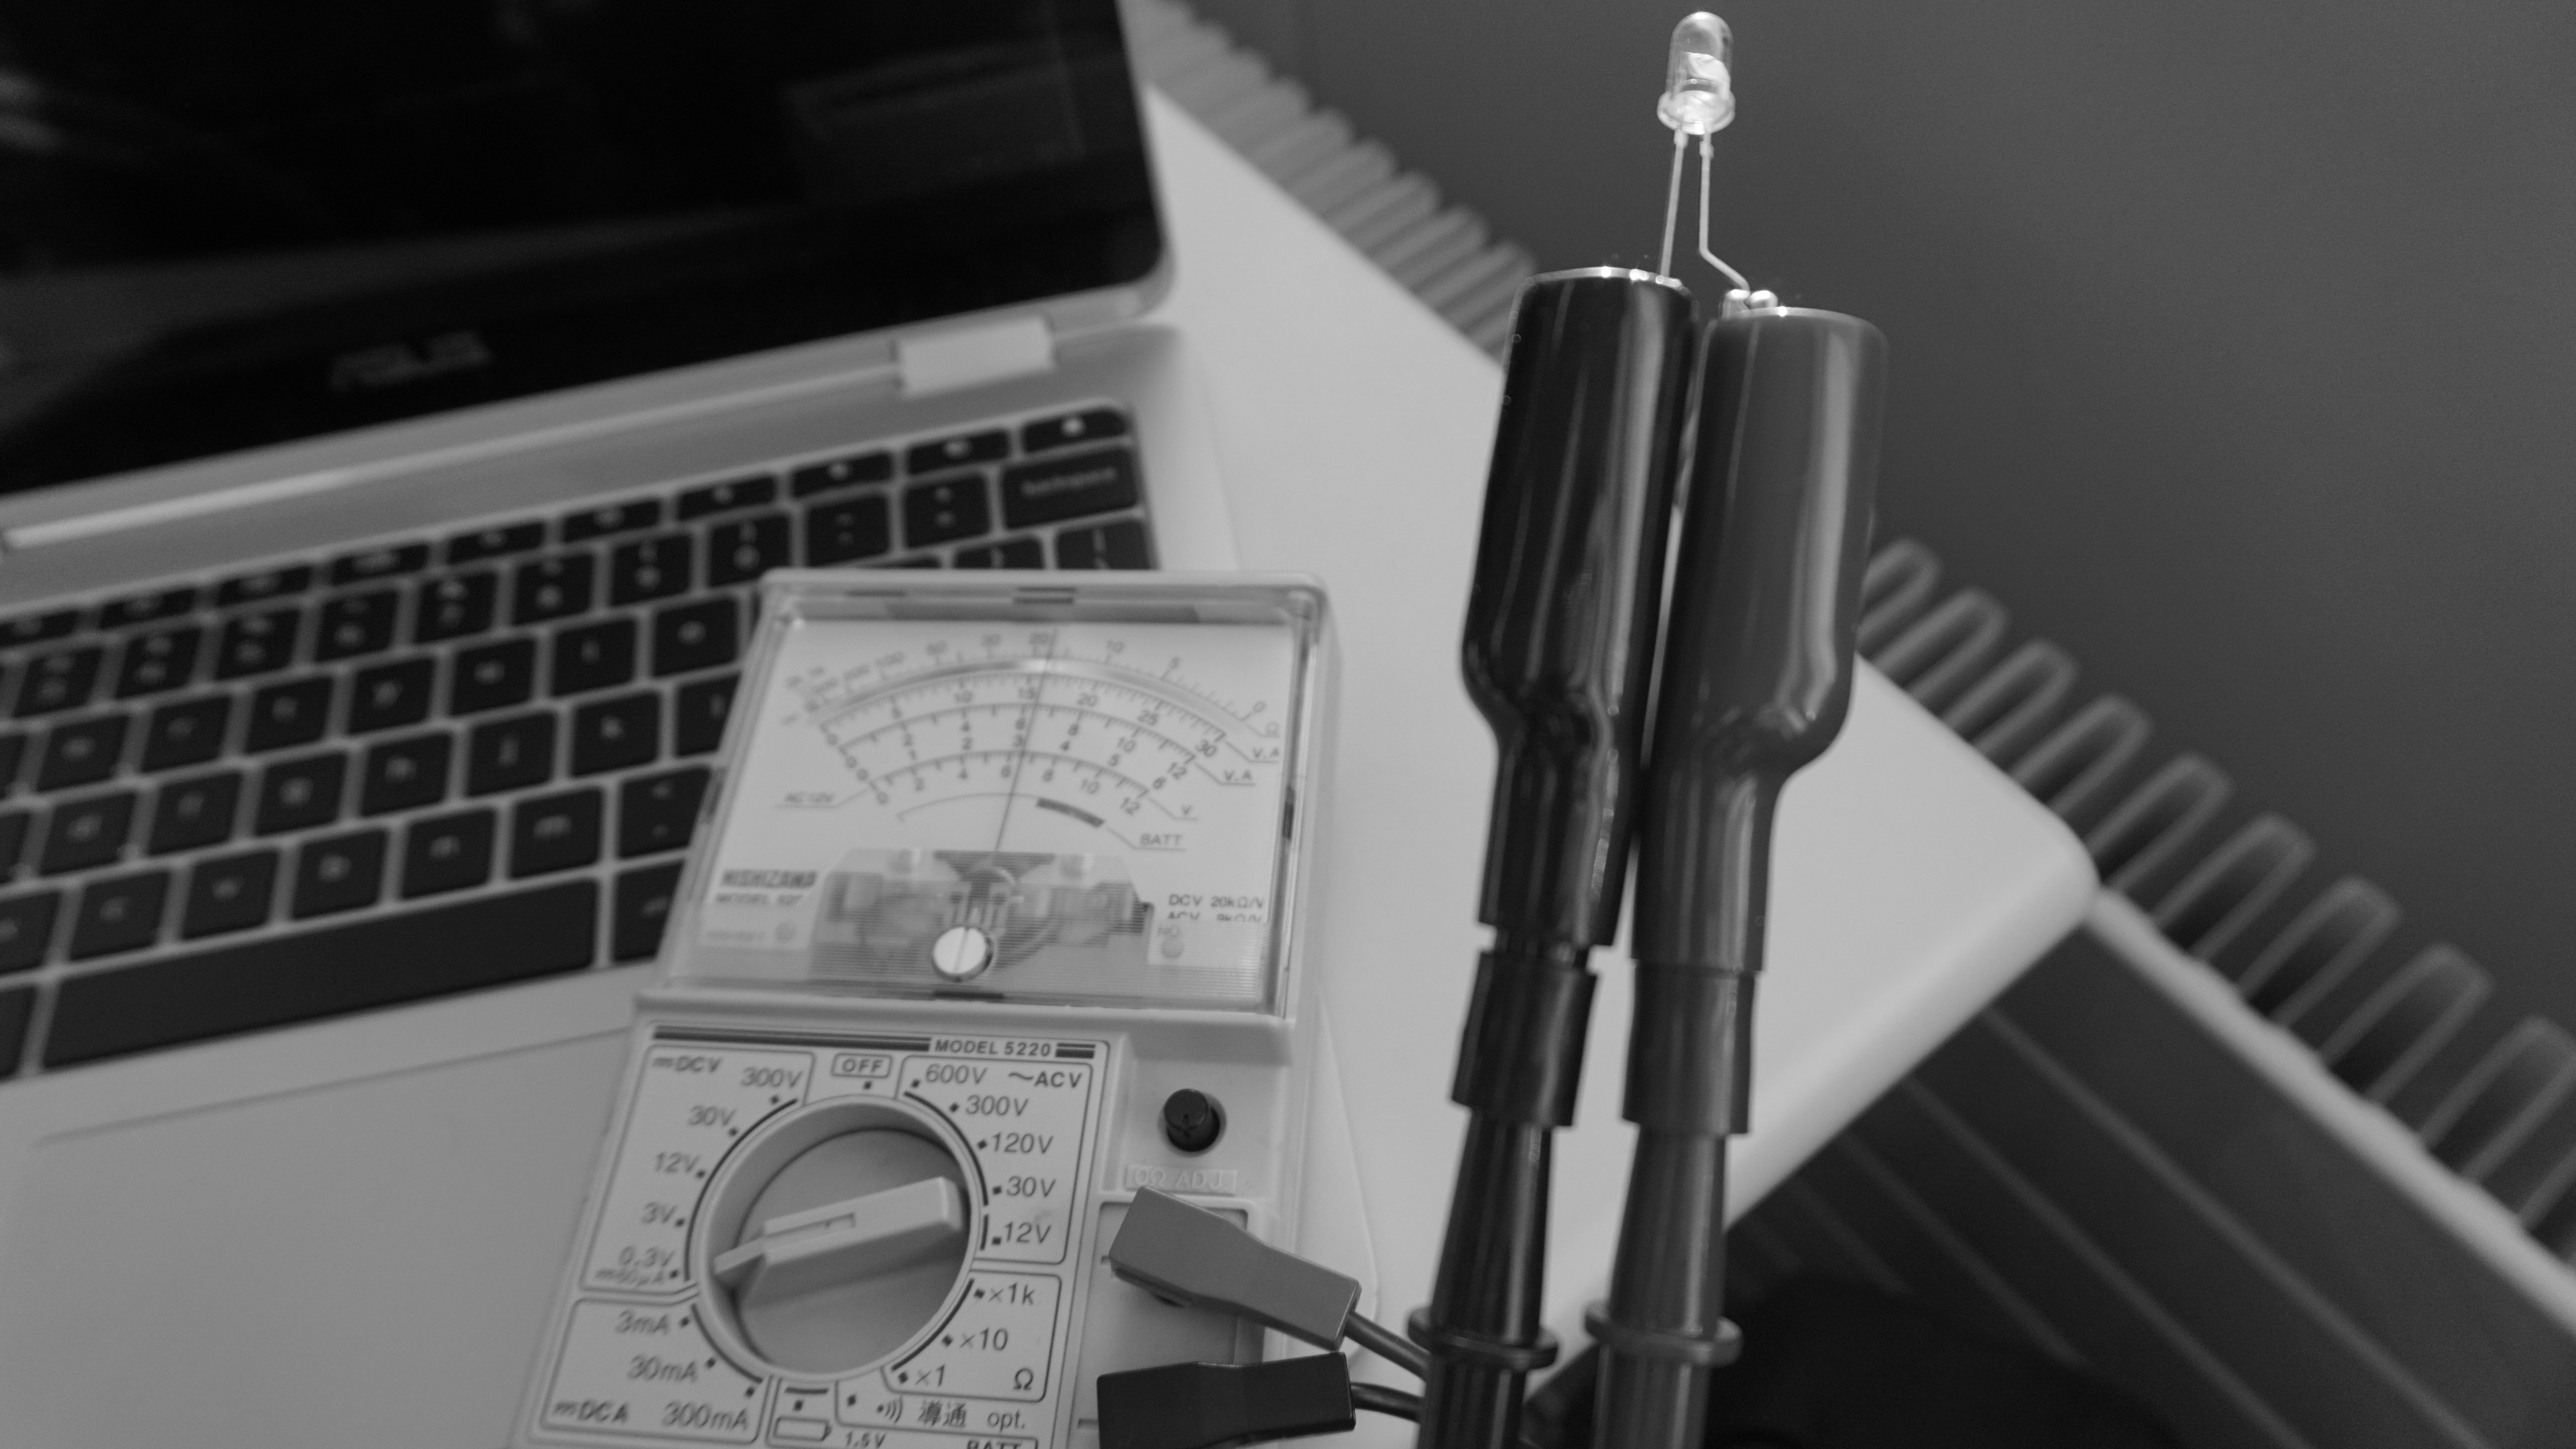
\includegraphics{./assets/mouse/1.JPG}
    \caption{LED1つのやつ}
    \label{fig:led1}
\end{figure}

\subsubsection{直列と並列どちらが良いのか考える}
先ほどはLED1個で発電してみましたが、次は複数接続してみたいと思います。
複数接続にあたり、直列接続と並列接続のどちらが発電に適しているのかを実験してみました。

\subsubsection{直列接続}
LED2個を直列に接続し、その両端をテスターで見ていきます。
そこに光を与えたところ、約100uA,約2.5V発生しました。
この結果から、LED1個の時と比べ、電流、電圧ともに2倍になっていることがわかります。

ぴんぼけしててごめんなさい
\begin{figure}[htbp]
    \centering
    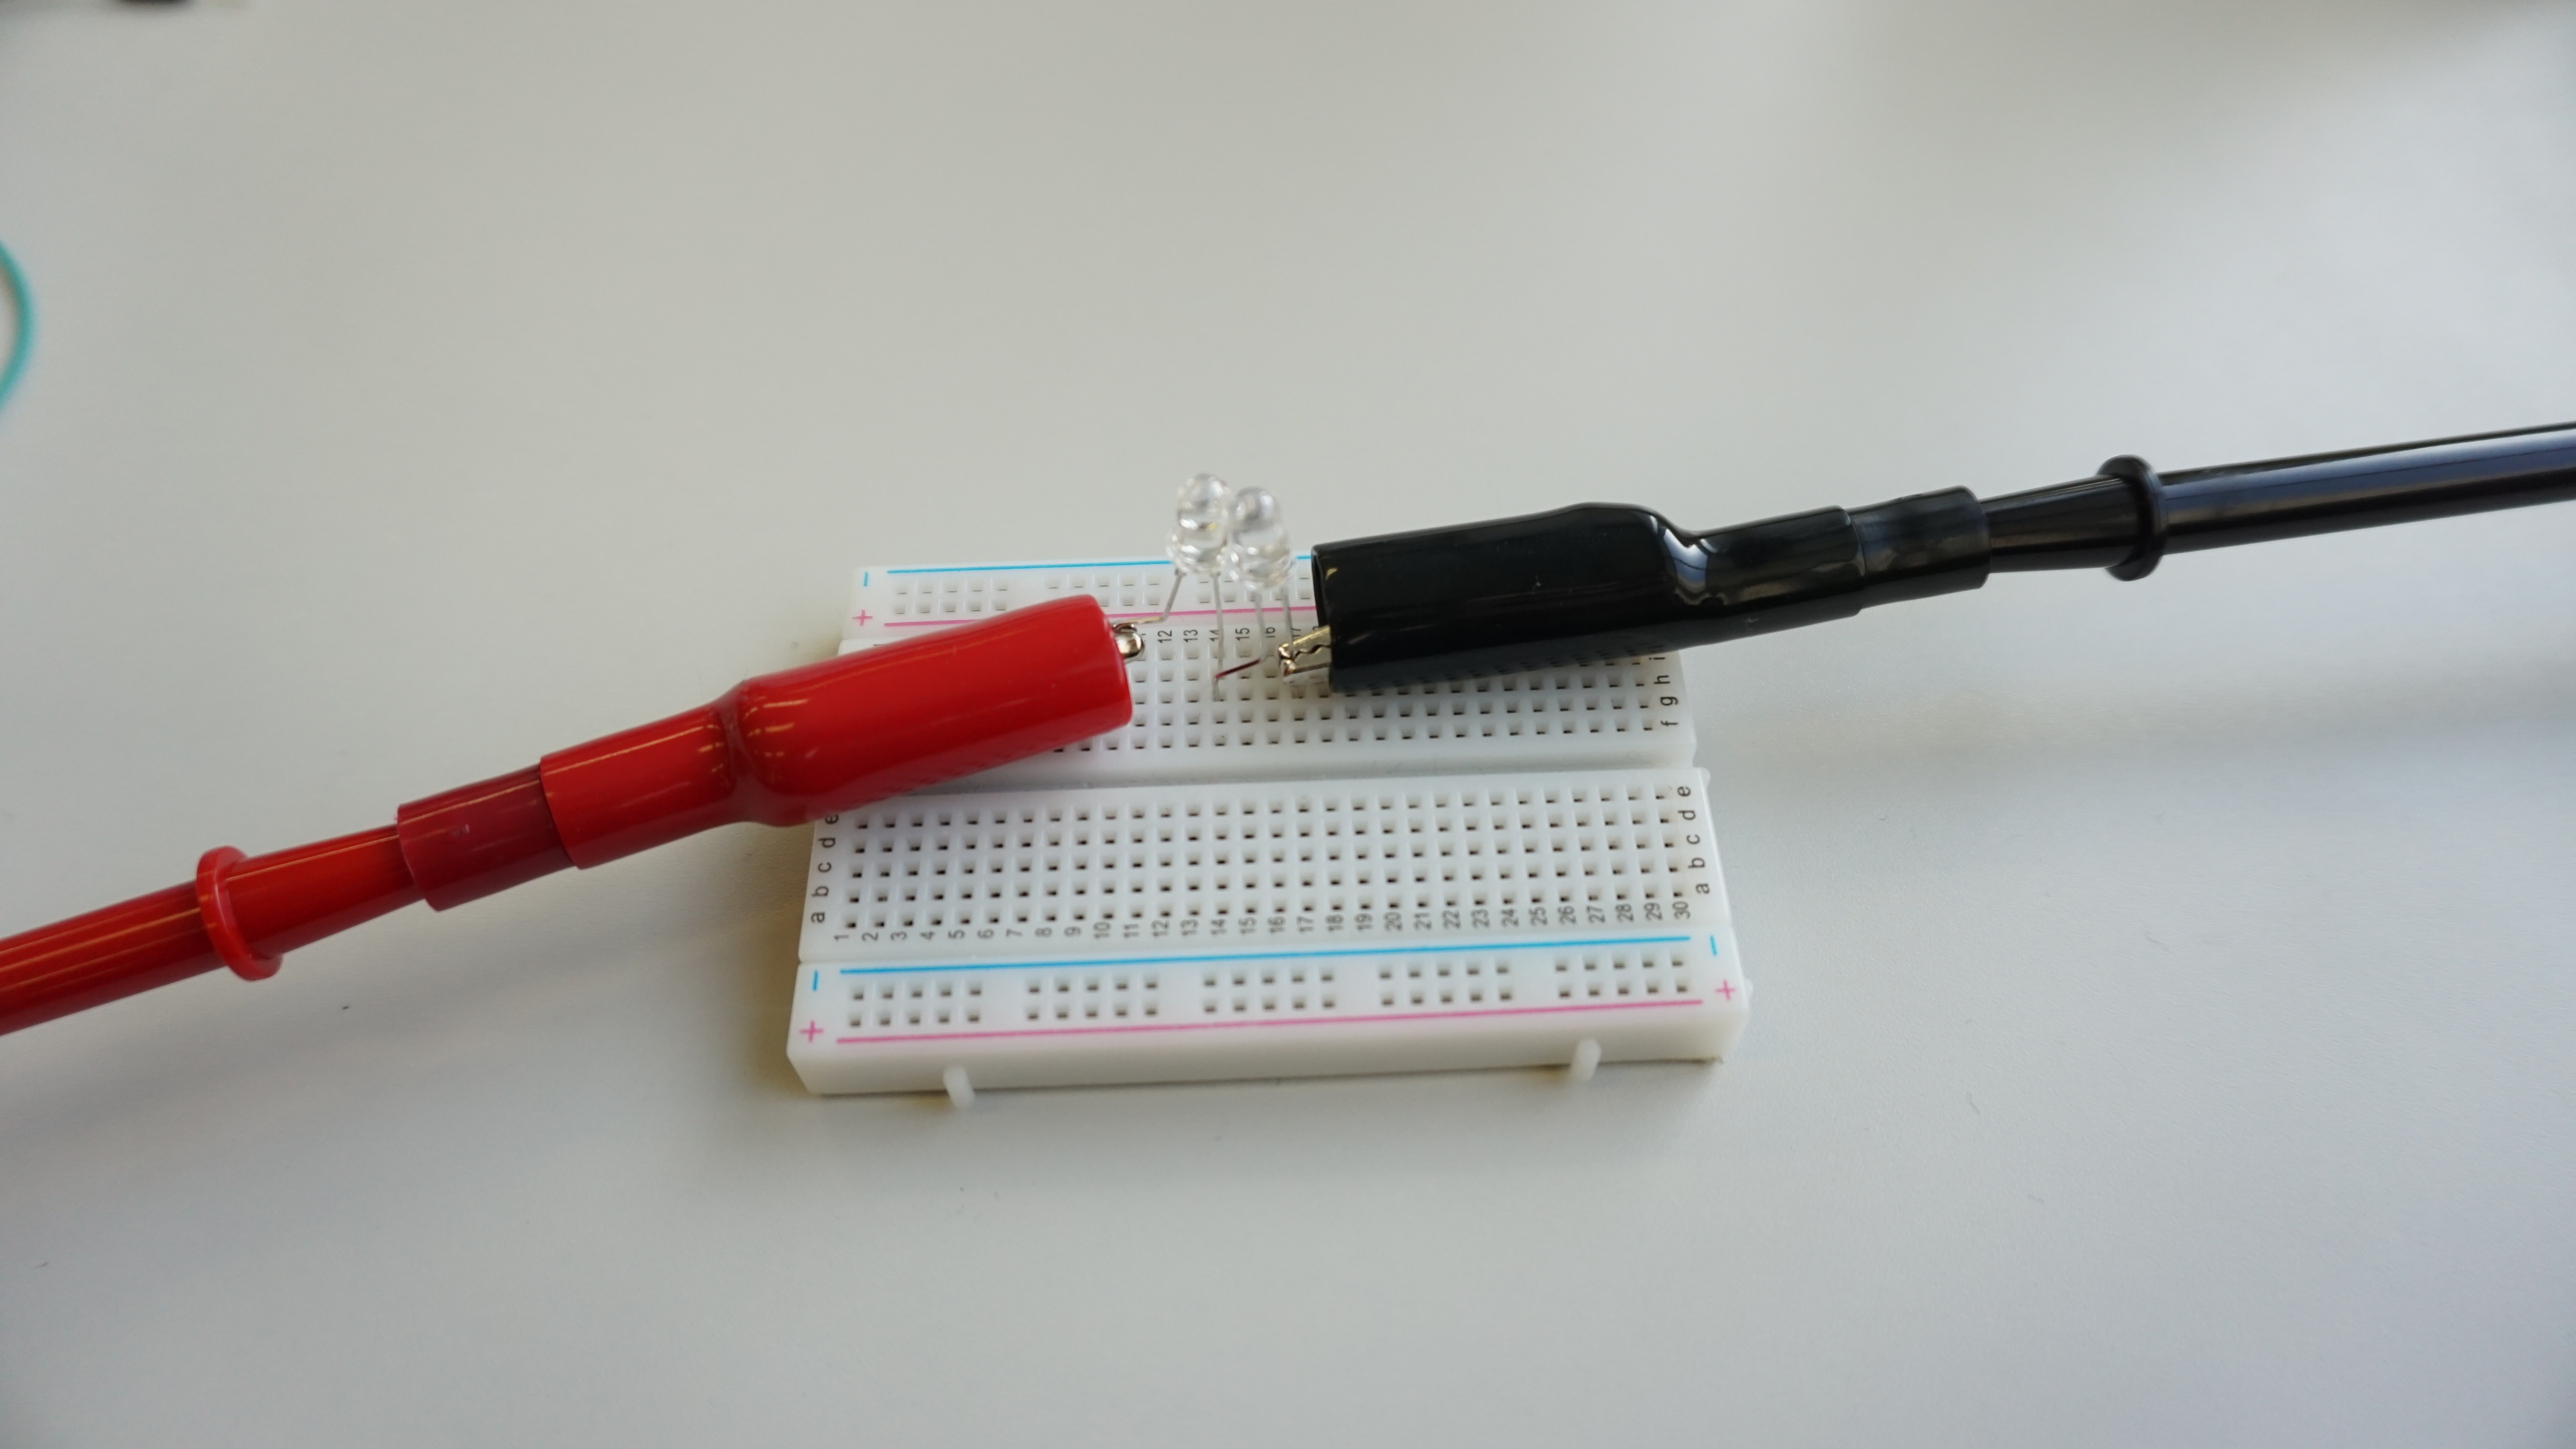
\includegraphics{./assets/mouse/12.JPG}
    \caption{LED2つ}
    \label{fig:led2}
\end{figure}

次にLED10個を直列に接続し、同じくその両端をテスターで見てみました。
その結果、約110uA,約0.5V発生しました。
LED2個の時と比べて電圧が極端に小さくなっていることがわかります。
これはおそらく、LEDの電圧降下の影響をもろに受けてしまったためだと思います。
電流値は、なんかいい感じです。


きっと並列のほうが綺麗に並ぶ
\begin{figure}[htbp]
    \centering
    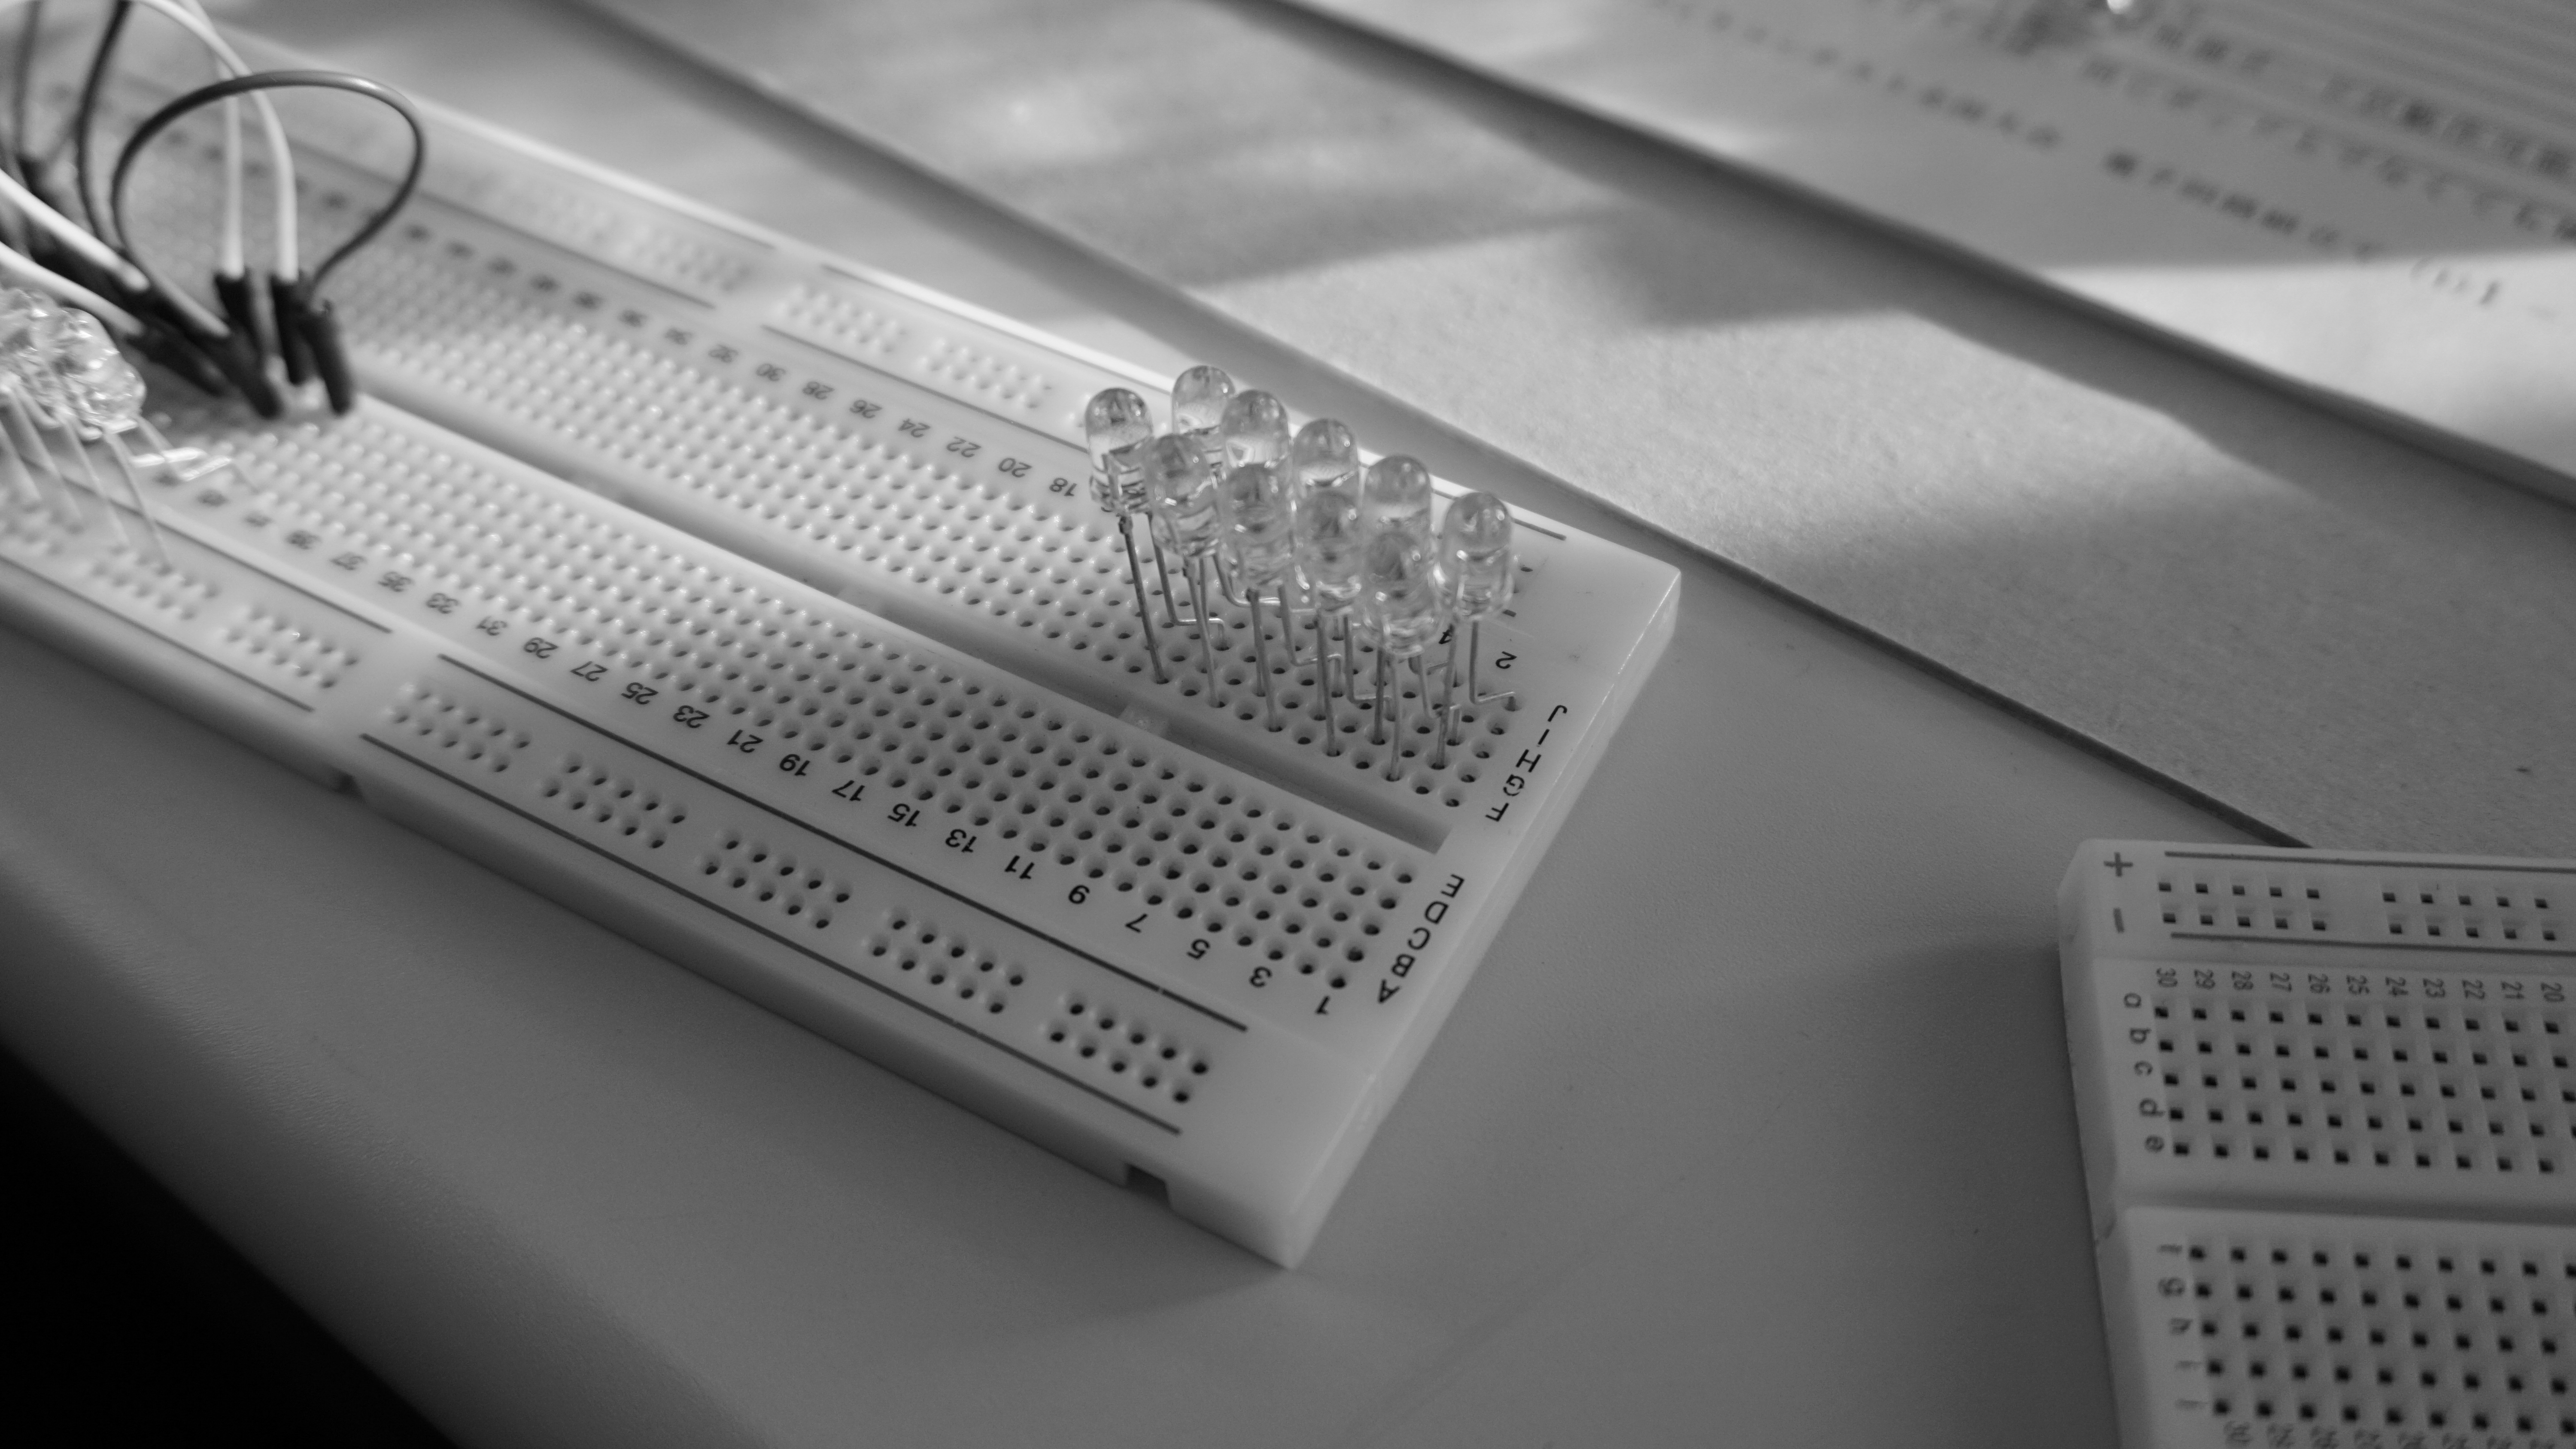
\includegraphics{./assets/mouse/4.JPG}
    \caption{LED10こ}
    \label{fig:led10}
\end{figure}

\subsubsection{並列接続}
LED2個数を並列に接続し、同じくテスターで見ていきます。
こちらも太陽光で、同じ時間帯に実験しました。
並列接続の場合、約100uA,1.5V発生しました。


なんか遠くてごめんんさい
\begin{figure}[htbp]
    \centering
    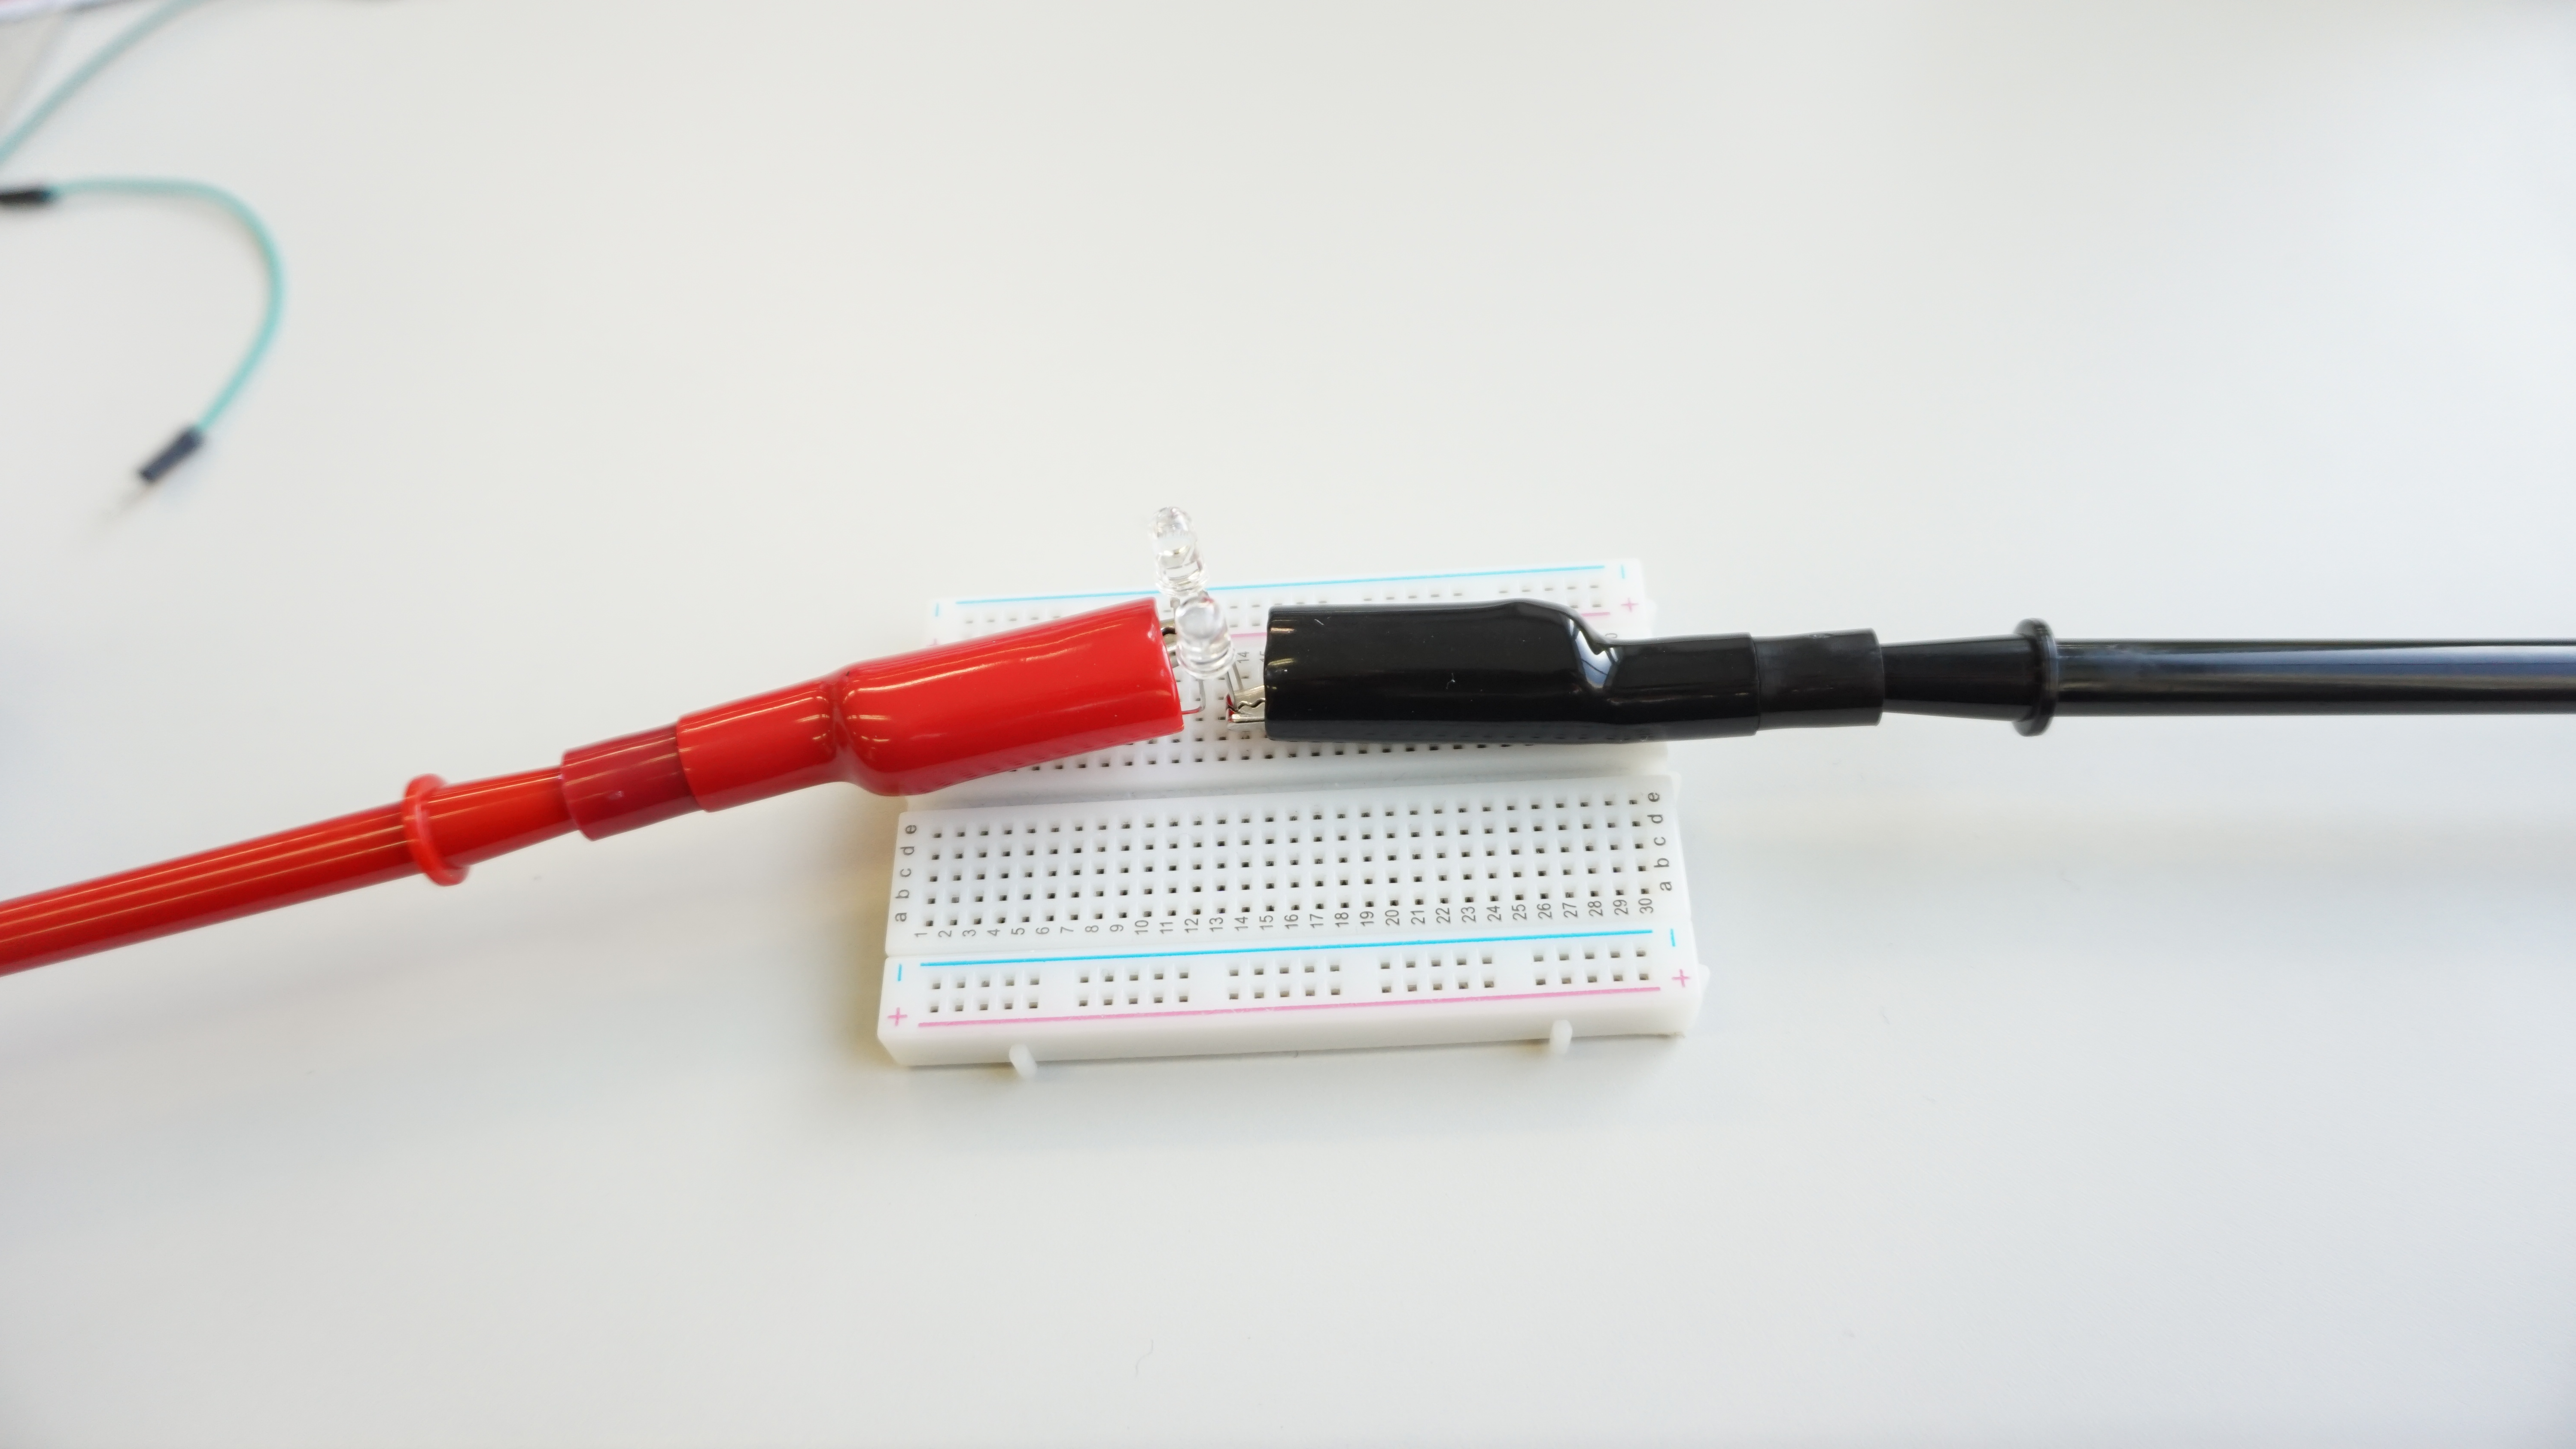
\includegraphics{./assets/mouse/13.JPG}
    \caption{LED並列}
    \label{fig:led_par}
\end{figure}


先ほどと同じく、LED10個を並列に並べたものの値を取っていきます。
こちらも同じく太陽光で、同じ時間帯です。
この環境で約0.4mA,1.5V発生しました。やっと現実味のある数値になってきました。
これは直列と違い抵抗が並列に接続されているためだと思われます。
よくわからないけどいきなり電流が大きくなりました。


やっぱり並列のほうが綺麗
\begin{figure}[htbp]
    \centering
    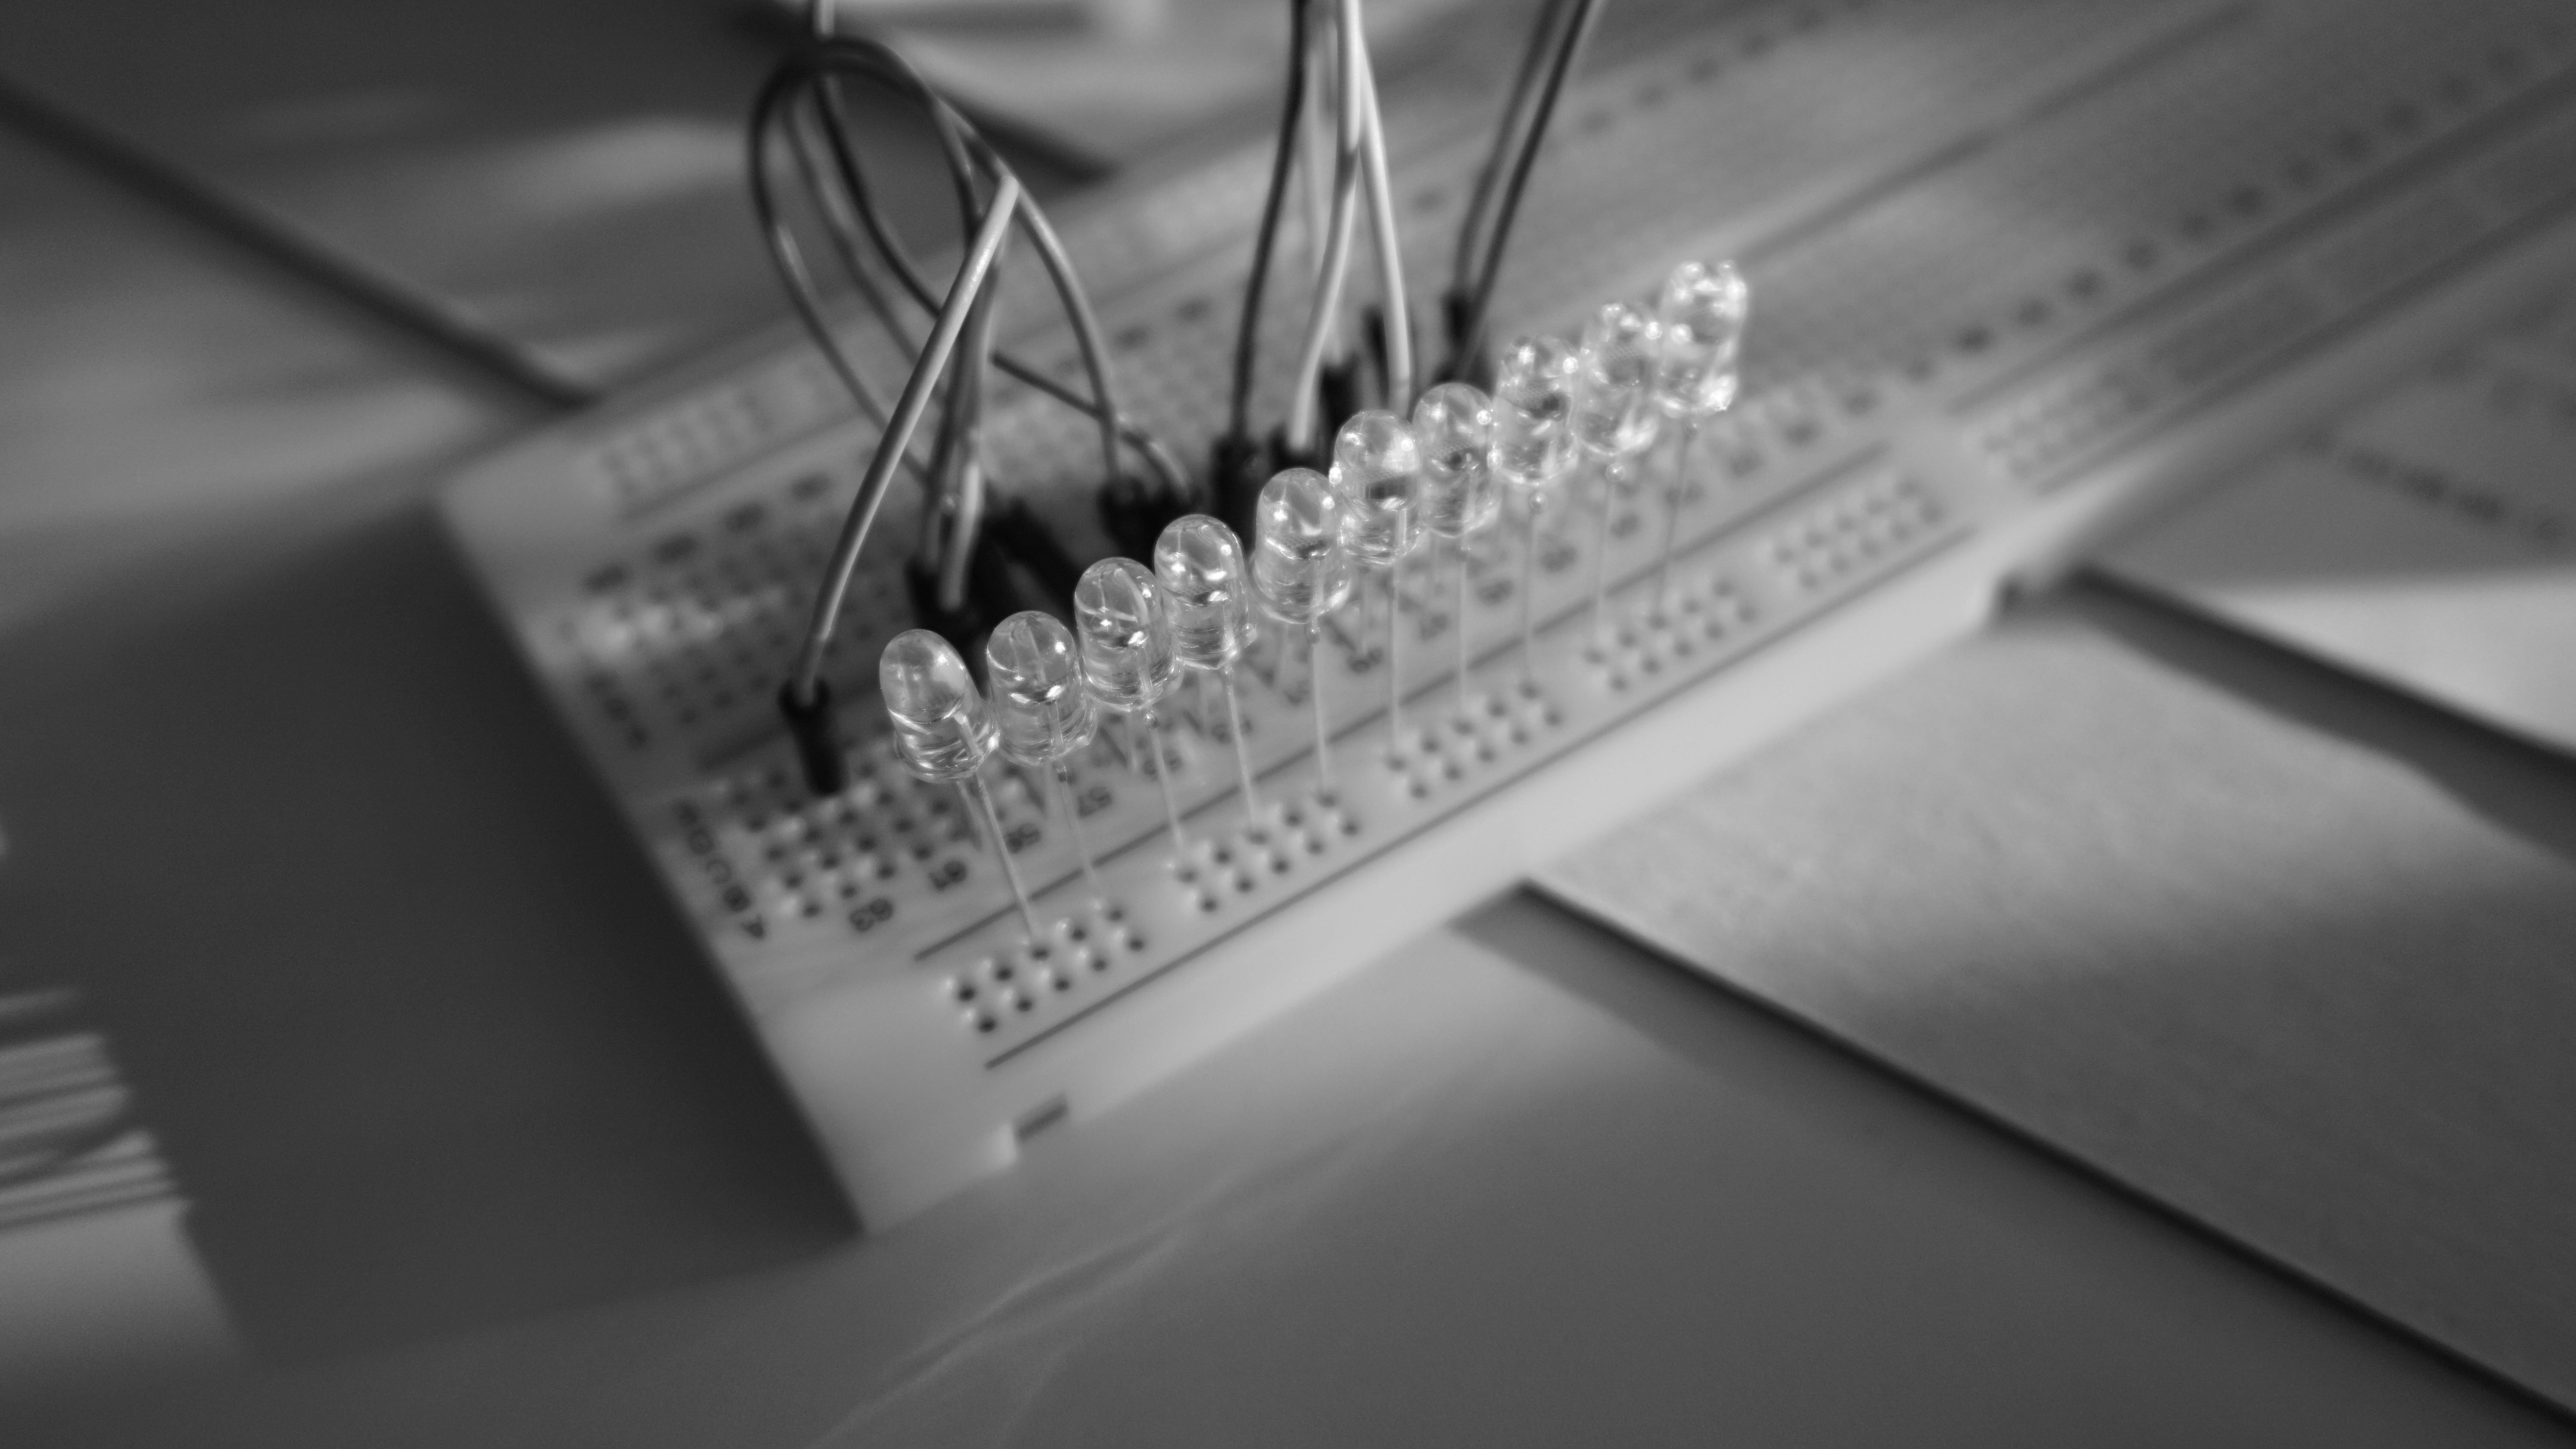
\includegraphics{./assets/mouse/5.JPG}
    \caption{LED10並列}
    \label{fig:led_par10}
\end{figure}

\subsubsection{結果}
直流と並列だと並列のほうが優秀だった
並列がなんでこうなったのかはよくわからないです。
とりあえず並列でのほうがLEDを光らせるのには現実的な発電量なので、

\subsection{LEDを30個並べる}
場所:ちかくの駐車場
時刻:14:30
光源:太陽光
照度:はかりわすれた

理論値だとLEDを30個並列に並べれば単純計算で1.2mA発生するはずです。
他の実験と同じ日に行いたかったのですが、太陽沈んでしまったので別の日に実験しました。

LEDを30個並べた様子(もうちょっとあるけど気にしないで)
\begin{figure}[htbp]
    \centering
    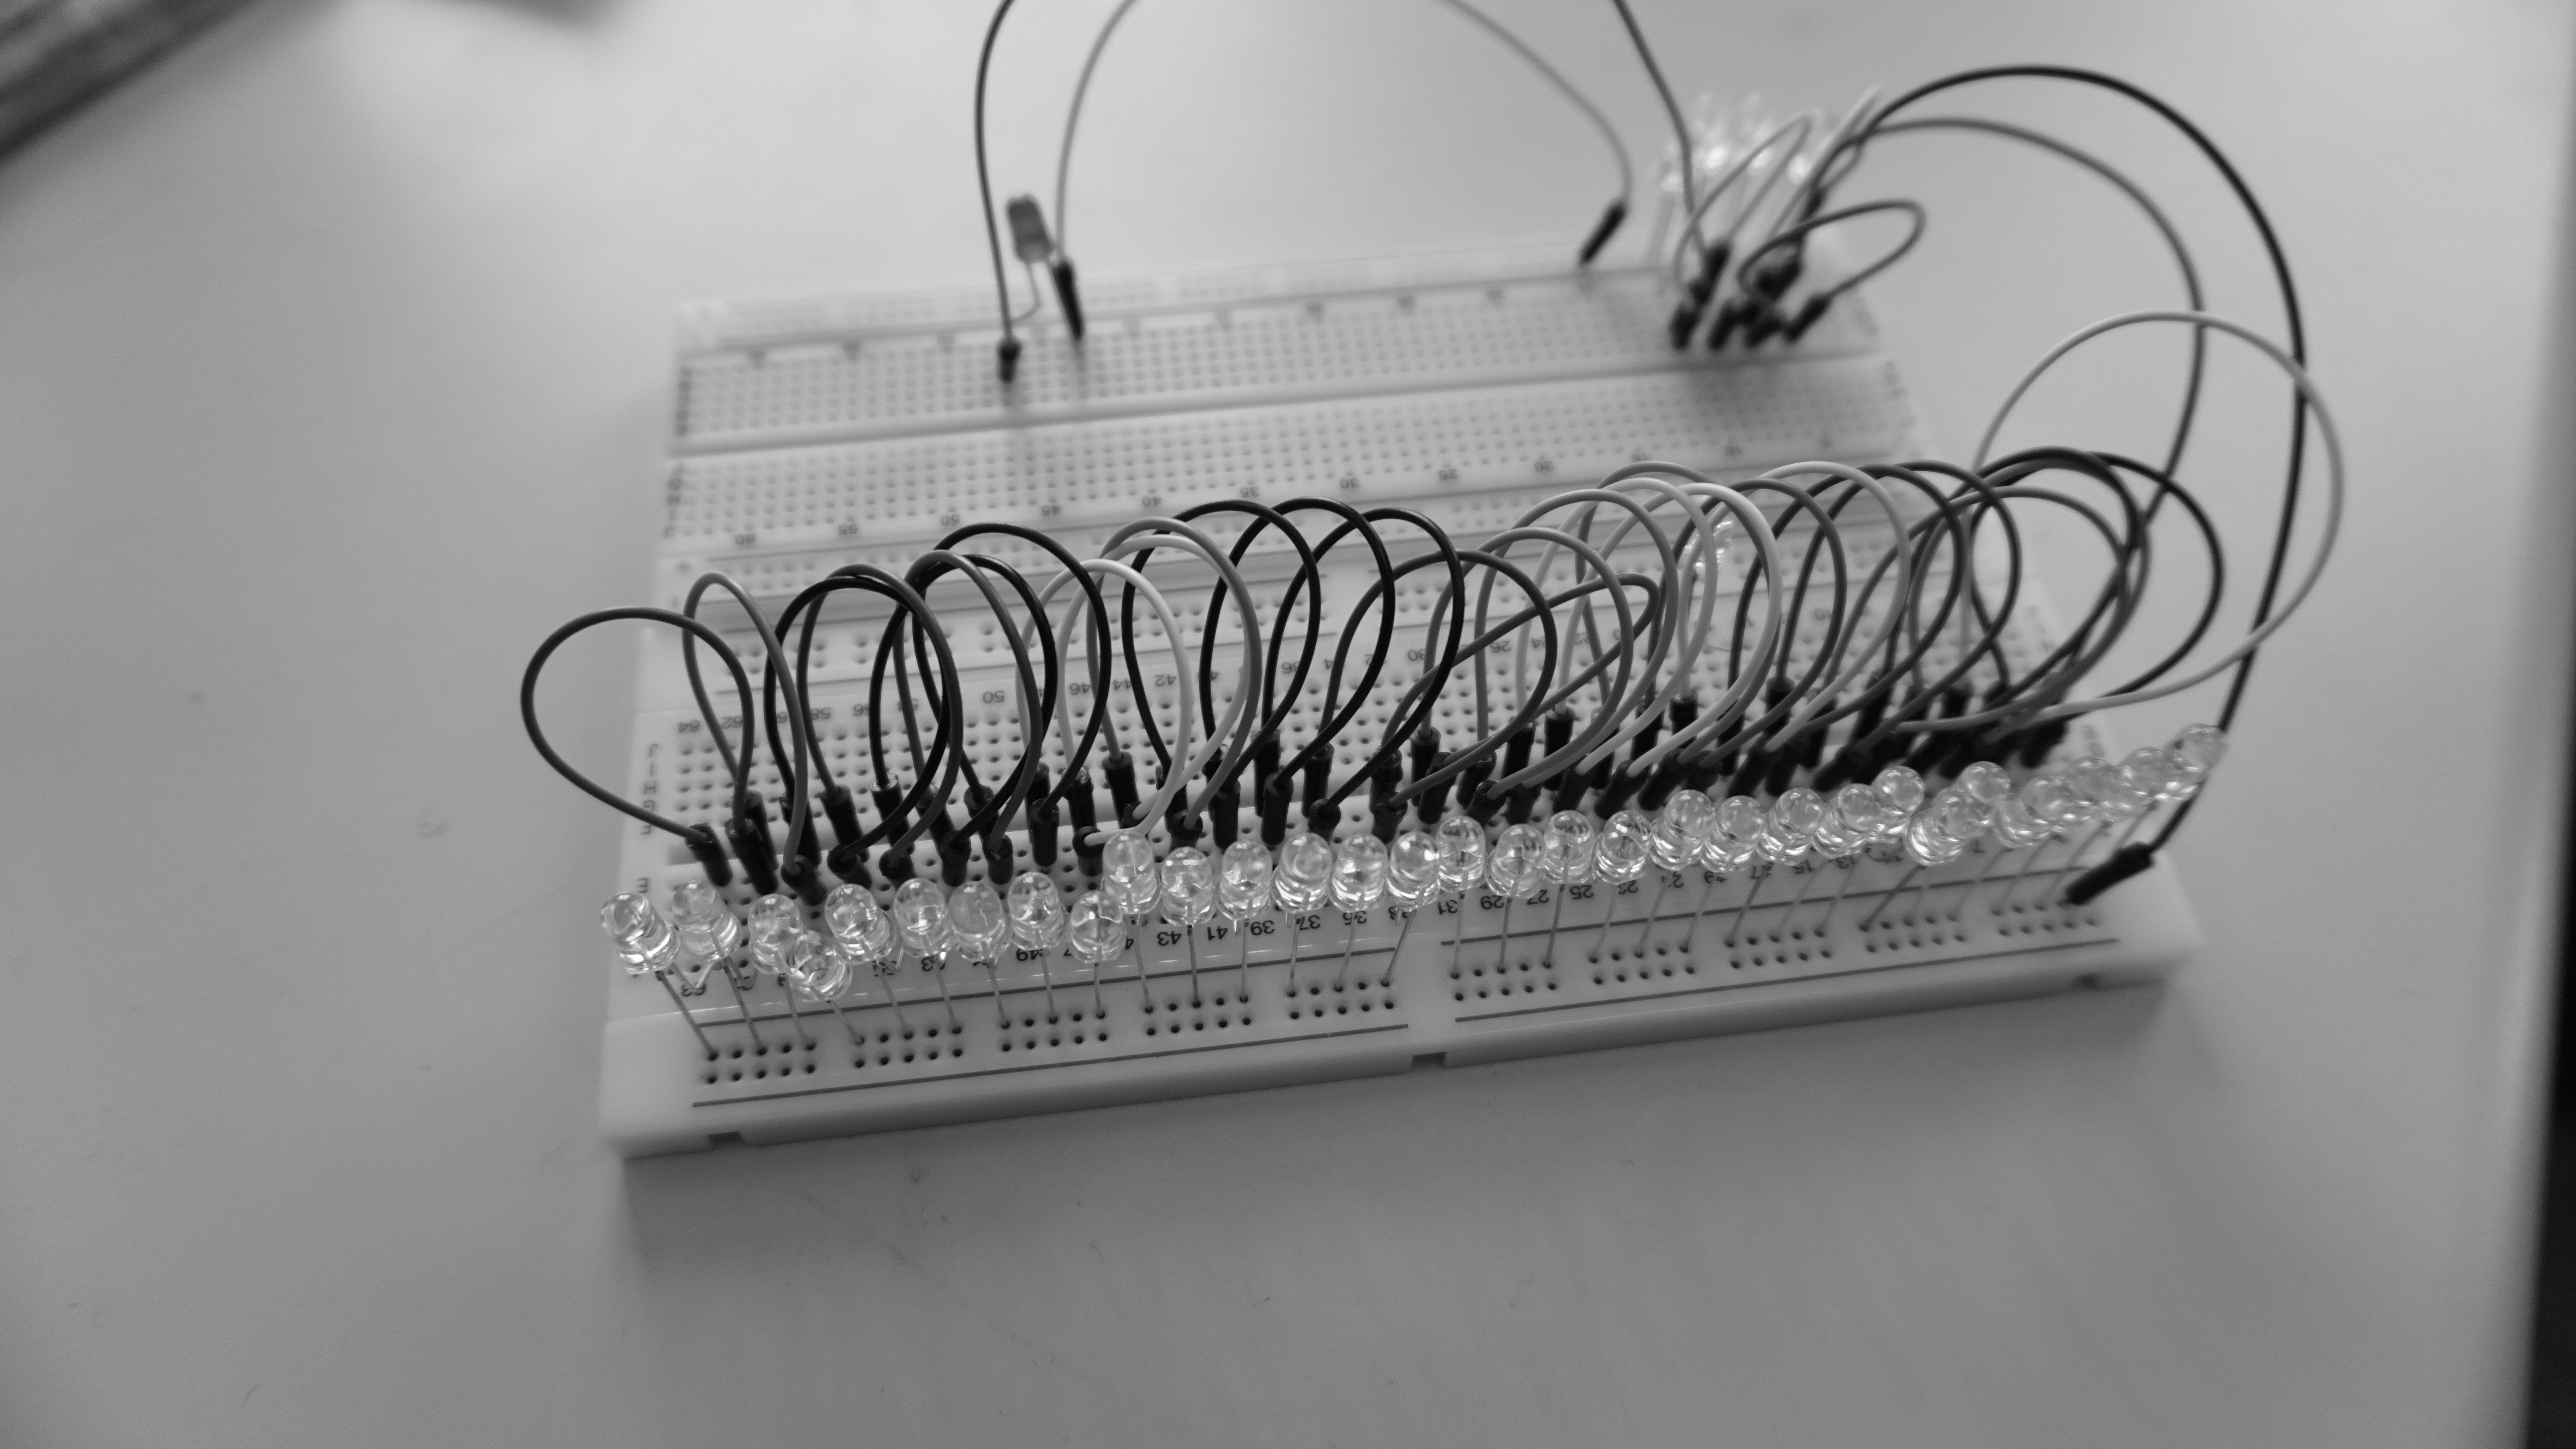
\includegraphics{./assets/mouse/10.JPG}
    \caption{LED30}
    \label{fig:led_par10}
\end{figure}

これをそのまま駐車場へ持って行き太陽の方へLEDを向けました。
この時は、約1mA,1.5Vとなりました。
1mAとはさわると少しぴりぴりするかしないか程度です。また、漏電も1mA以下が許容範囲です。つまり30個並列に並べて発生した電流は漏電にもならないのです。
悲しいですね。

\subsubsection{波長特性}
LEDにも波長特性はあります。
なので、LEDの色によって発電量も変わってきますし、光源の波長特性によっても全然違います。
場所、光源、LEDをしっかり選ぶとより良い発電ができるかもしれません。

\subsubsection{最後に}
LEDで発電するのはあまりお勧めできません。
まともに使おうとしたらたくさん並べなければいけないので、とてもめんどくさいです。
だけど僕はLEDで発電することに喜びを感じているので、これからもLEDで発電していこうとおもいます。
